\section{Introduction}
%----------------------------------------------------------------------
%----------------------------------------------------------------------
\begin{frame}[c]{Global Optimization}
Consider a 'well behaved' function $\cost$ : $\pcs \rightarrow \realnum$ where $\pcs \subseteq \realnum^D$ is a bounded domain.
\begin{equation*}
  \conf=\argmin_{\conf\in\pcs} \cost(\conf) 
\end{equation*}
\begin{figure}
   \begin{multicols}{2}
    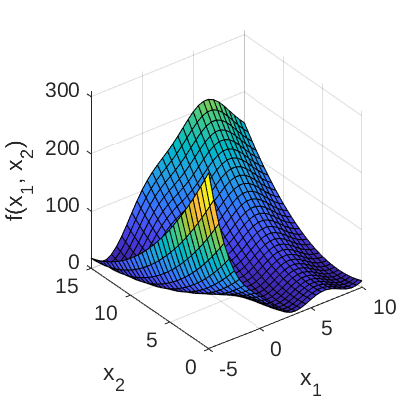
\includegraphics[width=0.2\textwidth, right]{images/intro_images/branin.png}
    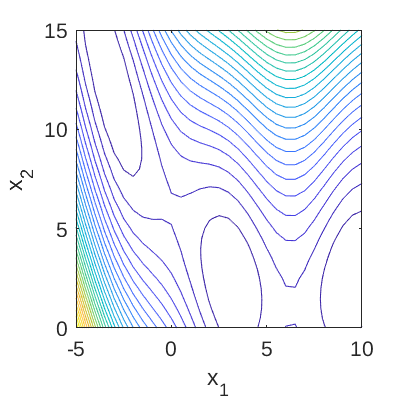
\includegraphics[width=0.2\textwidth,left]{images/intro_images/branin_countour.png}
 \end{multicols}
\end{figure}
\begin{itemize}
    \item Function $\cost$ is explicitly unknown and multimodal
    \item Only interaction: Query of function $\conf$ to obtain $\cost(\conf)$
    \item Evaluations of $\cost$ may be noisy
    \item Evaluations of $\cost$ are expensive
\end{itemize}

\tiny{\source{https://uqworld.org/} }


\end{frame}

%----------------------------------------------------------------------
%----------------------------------------------------------------------
%\begin{frame}[c]{Optimization problem example}

%We know that:
%\begin{itemize}
%    \item The function $\cost$ is Lipschitz continuous and differentiable.
%    \pause
%    \item The minimizer of $\cost$ is in the interval [0,1].
%    \pause
%    \item We have observed 3 evaluations of $\cost$.
%\end{itemize}

%\end{frame}
%----------------------------------------------------------------------
%\begin{frame}[c]{Problem description}
%\framesubtitle{We have 4 function evaluations}
%\begin{figure}
%    \centering
%    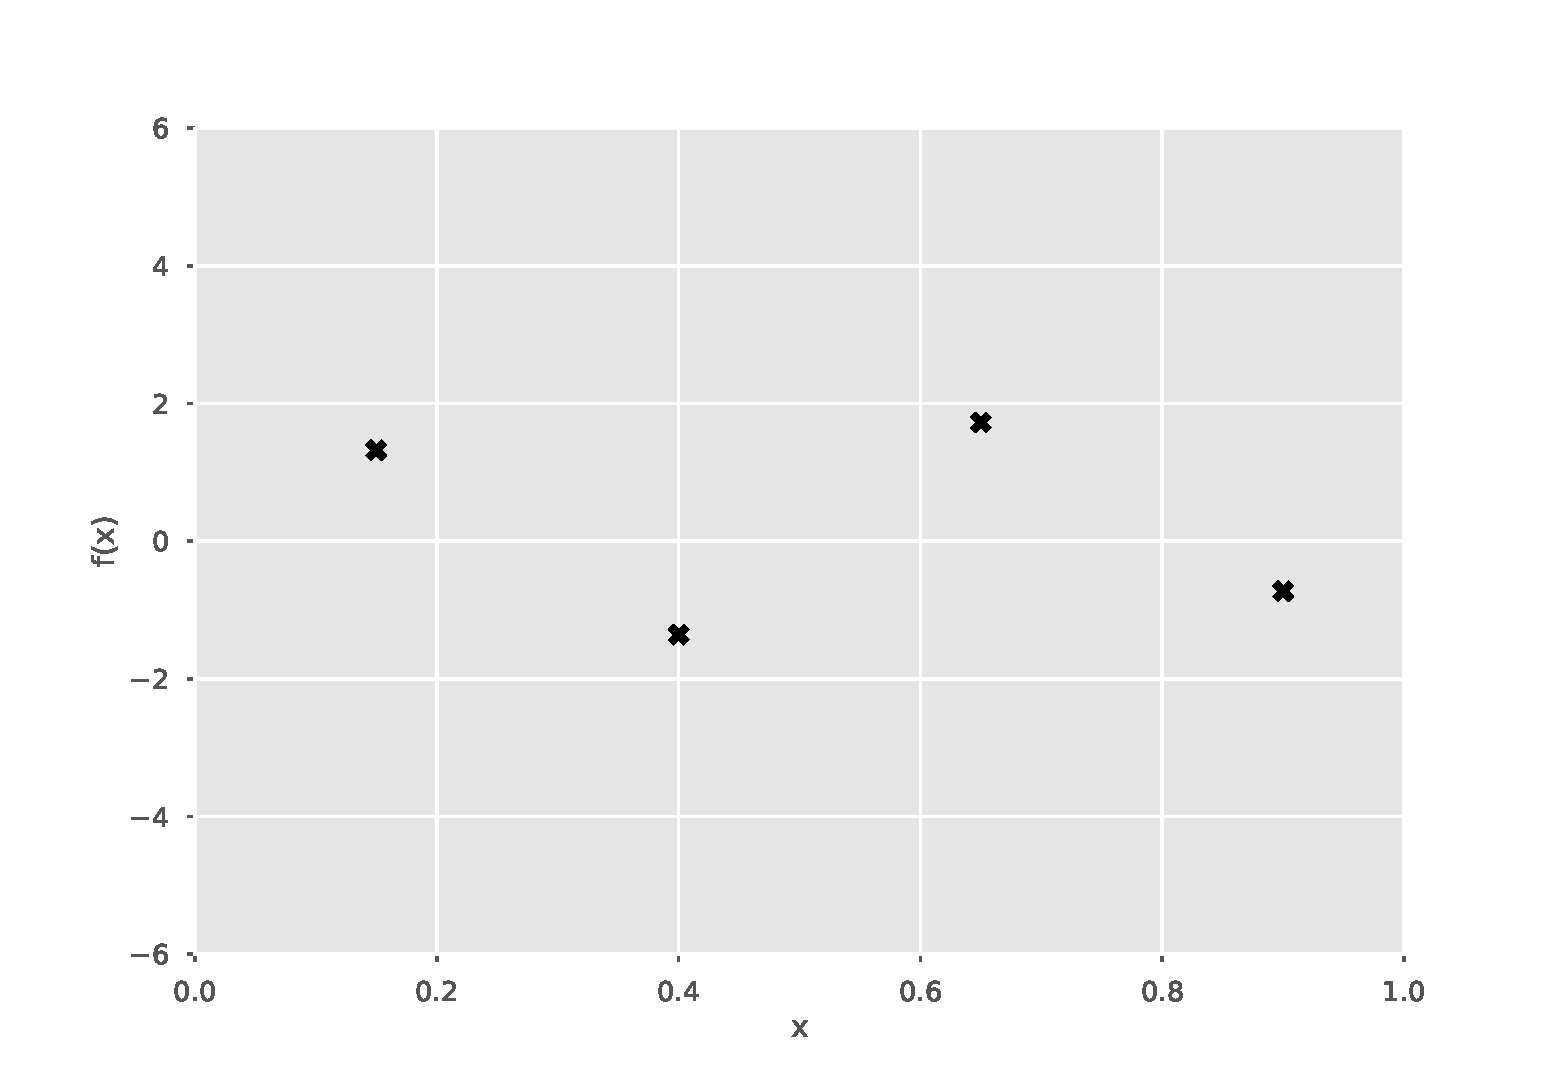
\includegraphics[width=0.8\textwidth, %height=0.38\textwidth]{images/intro_images/plot_datapoints.p%df}
%    \label{fig:my_label}
%\end{figure}
%\begin{center}
%  Where is the minimum of function $f$?  
%\end{center}
%\source{Plots are based on Javier Gonz\'alez's BO lecture %(bo\_intro.py)}



%\end{frame}

%-----------------------------------------------------------------------
%----------------------------------------------------------------------
%\begin{frame}[c]{Problem description}
%\framesubtitle{One possible curve}
%\begin{figure}
%    \centering
%    \includegraphics[width=0.7\textwidth, %height=0.4\textwidth]{images/intro_images/plot_posterior_1_s%ample.pdf}
%    \label{fig:my_label}
%\end{figure}
%\source{Plots are based on Javier Gonz\'alez's BO lecture %(bo\_intro.py)}



%\end{frame}

%-----------------------------------------------------------------------
%----------------------------------------------------------------------
%\begin{frame}[c]{Problem description}
%\framesubtitle{Three possible curves}
%\begin{figure}
%    \centering
%    \includegraphics[width=0.7\textwidth, %height=0.4\textwidth]{images/intro_images/plot_posterior_3_s%ample.pdf}
%    \label{fig:my_label}
%\end{figure}
%\source{Plots are based on Javier Gonz\'alez's BO lecture %(bo\_intro.py)}



%\end{frame}

%-----------------------------------------------------------------------
%----------------------------------------------------------------------
%\begin{frame}[c]{Problem description}
%\framesubtitle{Ten possible curves}
%\begin{figure}
%    \centering
%    \includegraphics[width=0.7\textwidth, %height=0.4\textwidth]{images/intro_images/plot_posterior_10_%sample.pdf}
%    \label{fig:my_label}
%\end{figure}
%\source{Plots are based on Javier Gonz\'alez's BO lecture %(bo\_intro.py)}



%\end{frame}

%-----------------------------------------------------------------------
%----------------------------------------------------------------------
%\begin{frame}[c]{Problem description}
%\framesubtitle{One hundred possible curves}
%\begin{figure}
%    \centering
%    \includegraphics[width=0.7\textwidth, %height=0.4\textwidth]{images/intro_images/plot_posterior_100%_sample.pdf}
%    \label{fig:my_label}
%\end{figure}
%\source{Plots are based on Javier Gonz\'alez's BO lecture %(bo\_intro.py)}



%\end{frame}

%-----------------------------------------------------------------------%----------------------------------------------------------------------
%\begin{frame}[c]{Problem description}
%\framesubtitle{One thousand possible curves}
%\begin{figure}
%    \centering
%    \includegraphics[width=0.7\textwidth, %height=0.4\textwidth]{images/intro_images/plot_posterior_100%0_sample.pdf}
%    \label{fig:my_label}
%\end{figure}
%\source{Plots are based on Javier Gonz\'alez's BO lecture (bo\_intro.py)}



%\end{frame}

%-----------------------------------------------------------------------
%----------------------------------------------------------------------
%\begin{frame}[c]{Problem description}
%\framesubtitle{Infinitely many curves}
%\begin{figure}
%    \centering
%    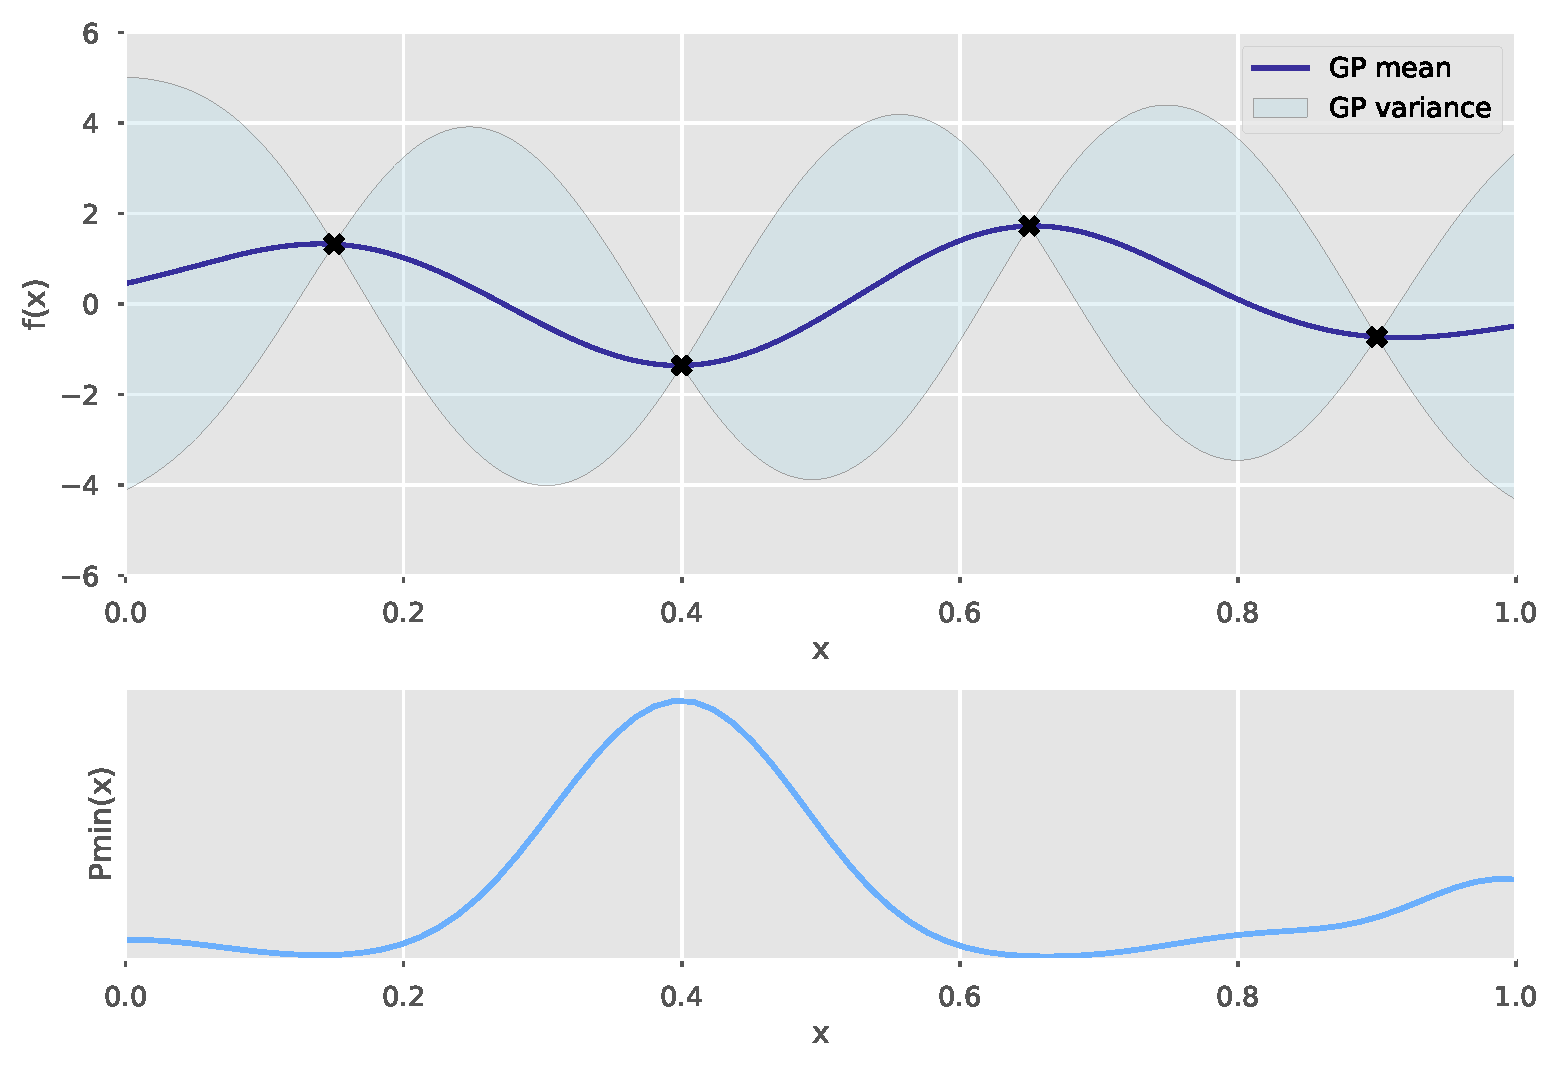
\includegraphics[width=0.7\textwidth, %height=0.4\textwidth]{images/intro_images/plot_posterior.pdf%}
%    \label{fig:my_label}
%\end{figure}
%\source{Plots are based on Javier Gonz\'alez's BO lecture (bo\_intro.py)}


%\end{frame}






%-----------------------------------------------------------------------
\myframe{Bayesian Optimization in a Nutshell}{
  
\vspace*{-0.5cm}
\begin{columns}[T]

\column{0.6\textwidth}

\myblock{General approach}{
	\myit{
	  \item Fit a probabilistic model to the collected function samples
	  $\langle{}\conf, f(\conf)\rangle{}$
	  \item Use the model to guide optimization, trading off
	  exploration \vs{} exploitation
	%  \item Acquisition function for exploration-exploitation tradeoff
	%  \item Optimize on acquisition function\\ to get next $x$
	  %$\conf$ ($x$)
	}
}

%\smallskip
\onslide<5->{
	\myblock{Popular approach in the statistics literature since \litw{\href{http://link.springer.com/chapter/10.1007\%2F3-540-07165-2_55}{Mockus,
	1978}}}{ \myit{
		  	\item Efficient in \# function evaluations 
		  	\item Works when objective is nonconvex, noisy, has unknown derivatives, etc
			\pause
			\item Recent convergence results\\ \lit{Srinivas et al, 2010; Bull 2011;
			de Freitas et al, 2012; Kawaguchi et al, 2015}
			%TODO: sorry, I don't know these papers
		%	\item Popular \alert{Bayesian optimization workshop} at NIPS (the premiere machine learning conference)
		}
	}
}

%\begin{enumerate}
%  \item Fit an empirical performance model (EPM) 
%  \item Acquisition function for exploration-exploitation tradeoff
%  \item Optimize on acquisition function\\ to get next $\conf$ ($x$)
%\end{enumerate}

\column{0.4\textwidth}
\vspace*{0.5cm}
\onslide<2->{
	%\includegraphics[width=1\textwidth]{../images/bo.png}
	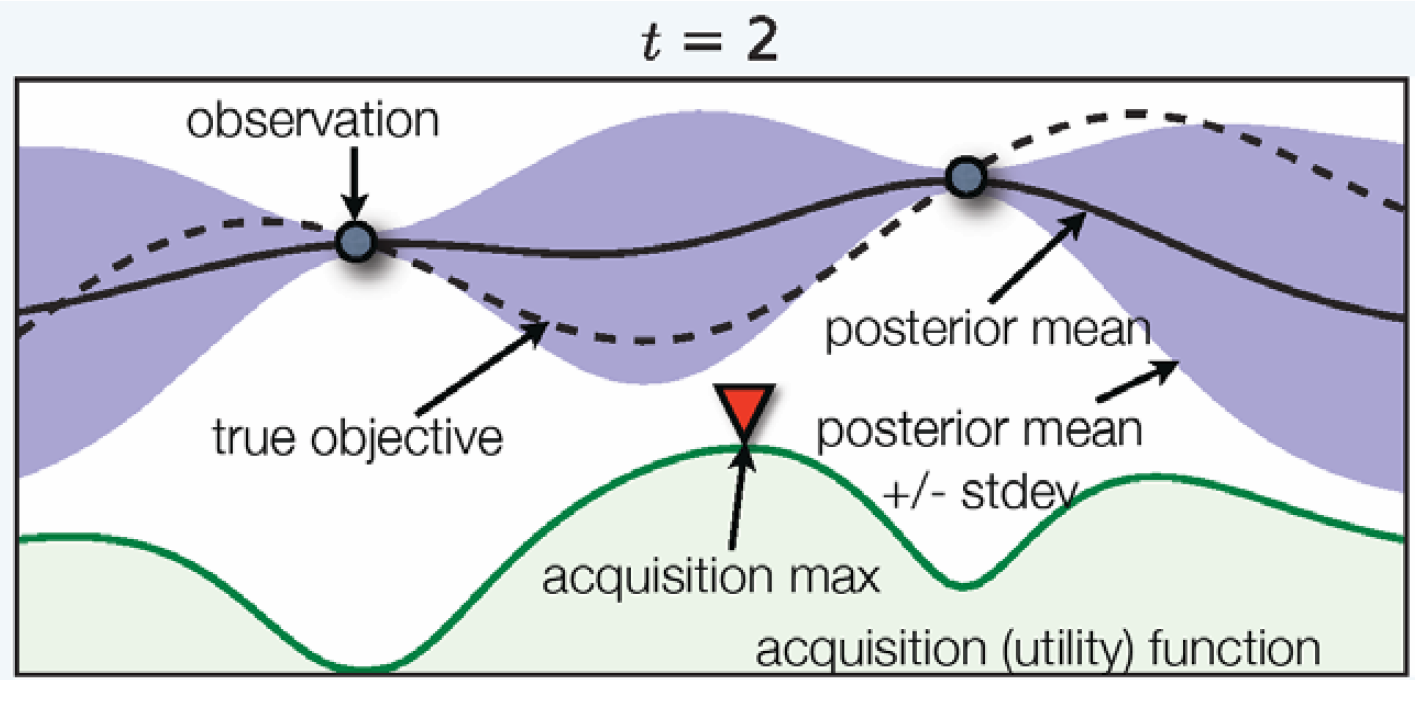
\includegraphics[width=0.9\textwidth]{plots_and_scripts/plots/bo_pic1.png}\\
	\pause
	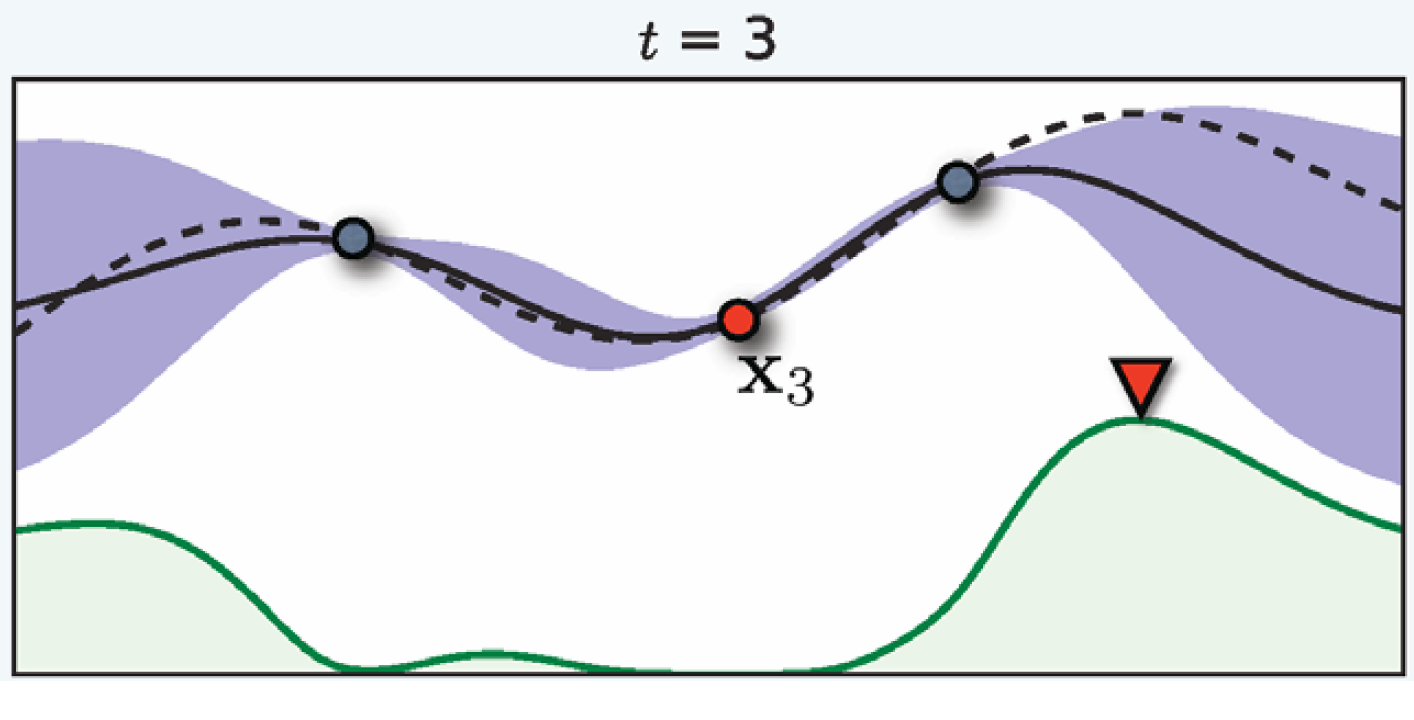
\includegraphics[width=0.9\textwidth]{plots_and_scripts/plots//bo_pic2.png}\\
	\pause
	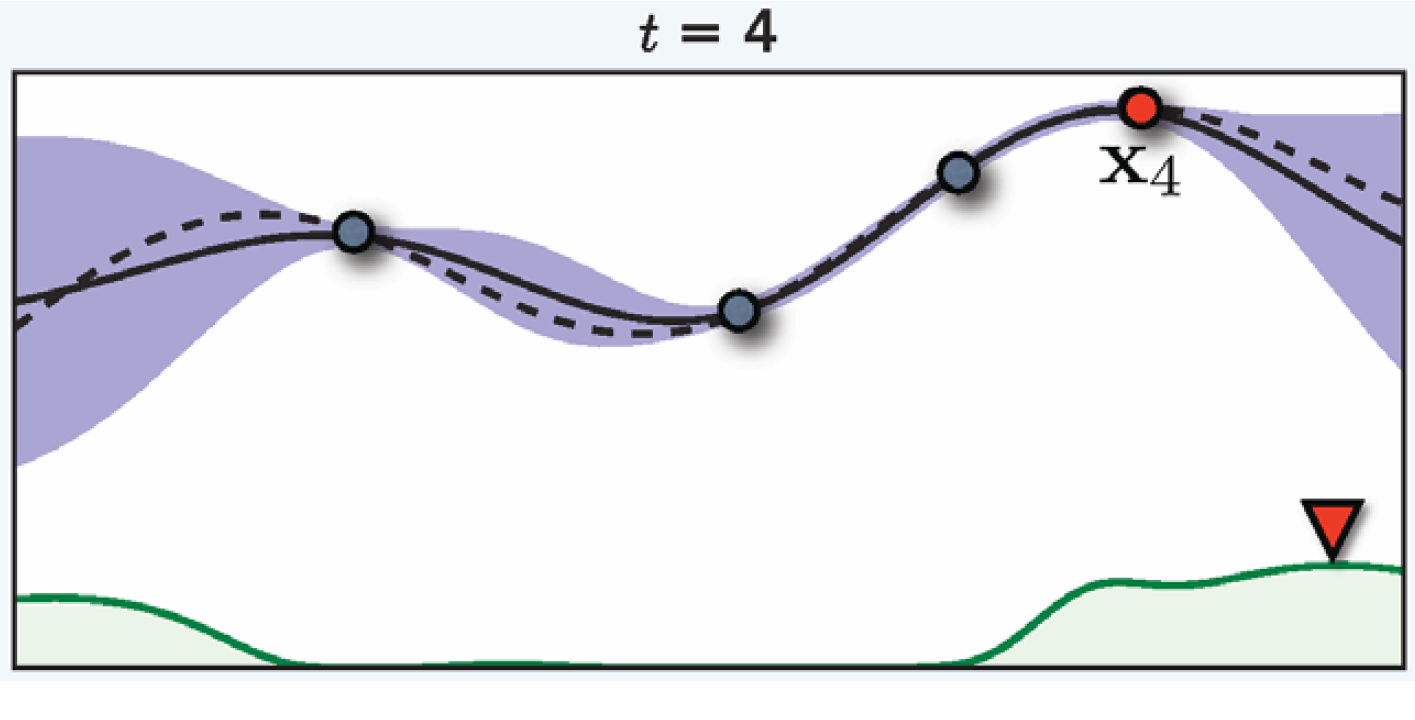
\includegraphics[width=0.9\textwidth]{plots_and_scripts/plots//bo_pic3.png}\\
	\footnotesize{Image source: \lit{\href{https://arxiv.org/abs/1012.2599}{Brochu et al, 2010}}}
}
\end{columns}


}
%-----------------------------------------------------------------------


%-----------------------------------------------------------------------
%----------------------------------------------------------------------
\begin{frame}[c]{Bayesian Optimization: Visualization of Many Steps}
\begin{figure}
    \centering
    \only<1>{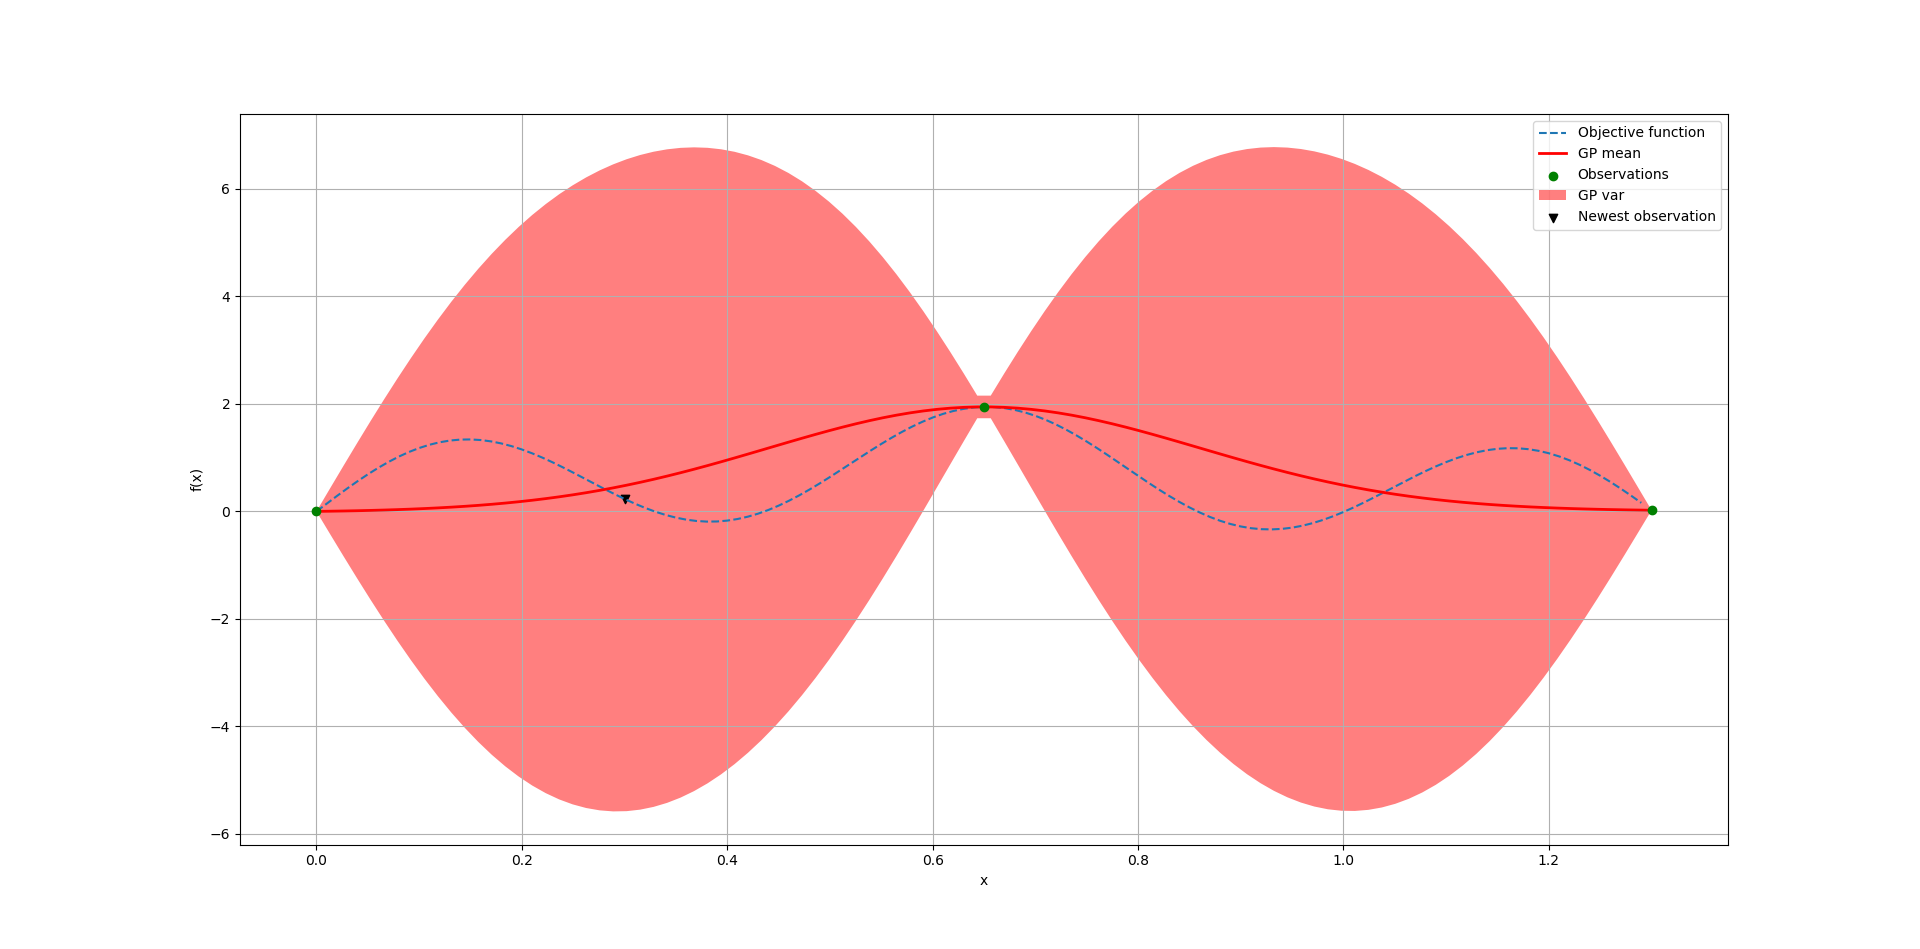
\includegraphics[width=\linewidth]{images/intro_images/BOLoop_1.png}}
    \only<2>{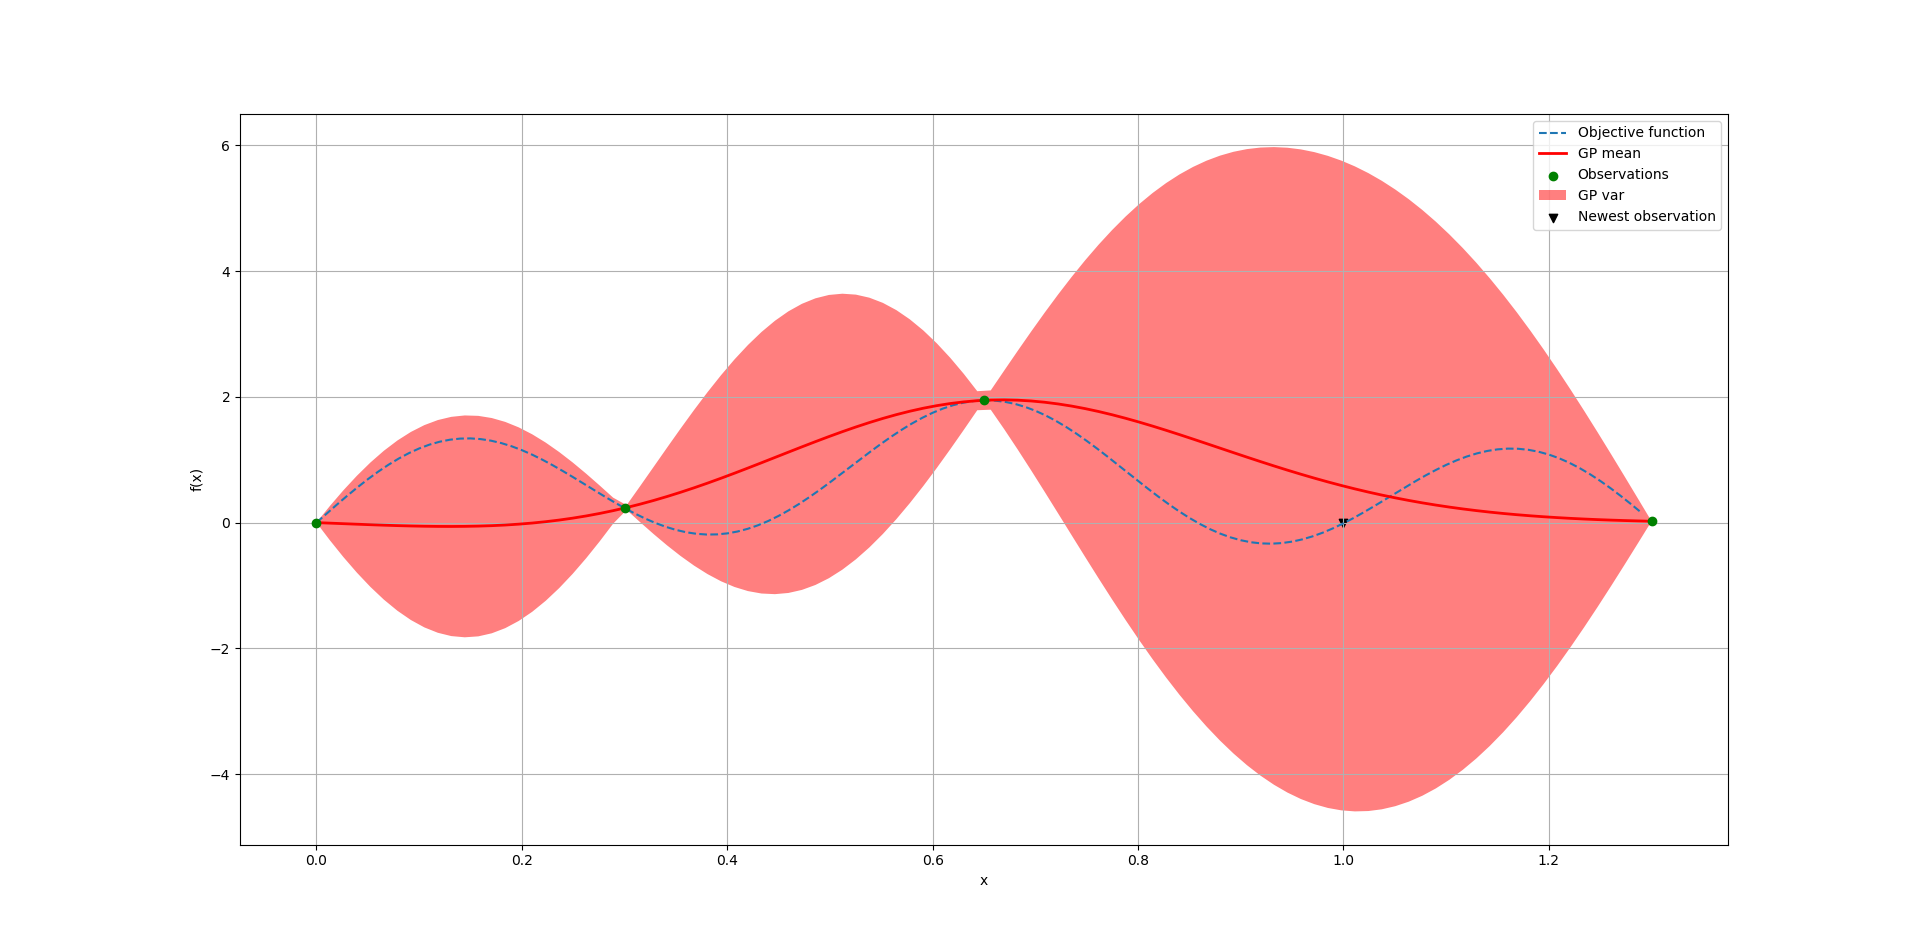
\includegraphics[width=\linewidth]{images/intro_images/BOLoop_2.png}}
    \only<3>{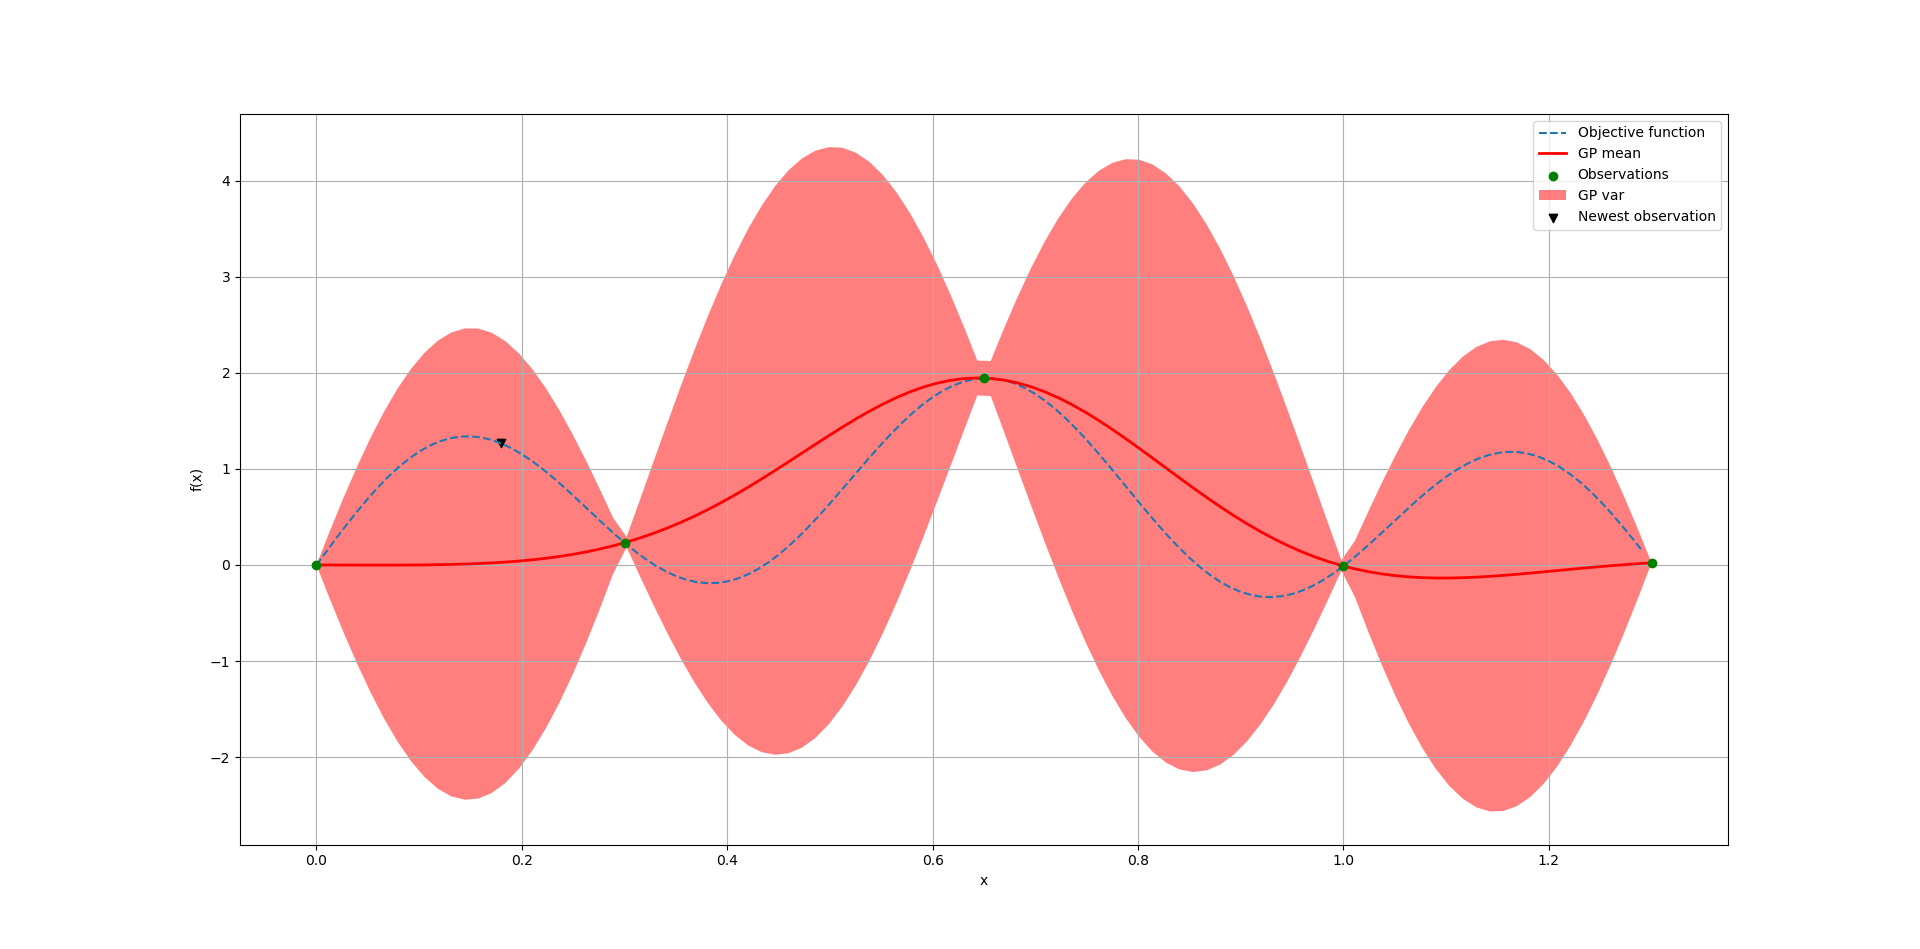
\includegraphics[width=\linewidth]{images/intro_images/BOLoop_3.png}}
    \only<4>{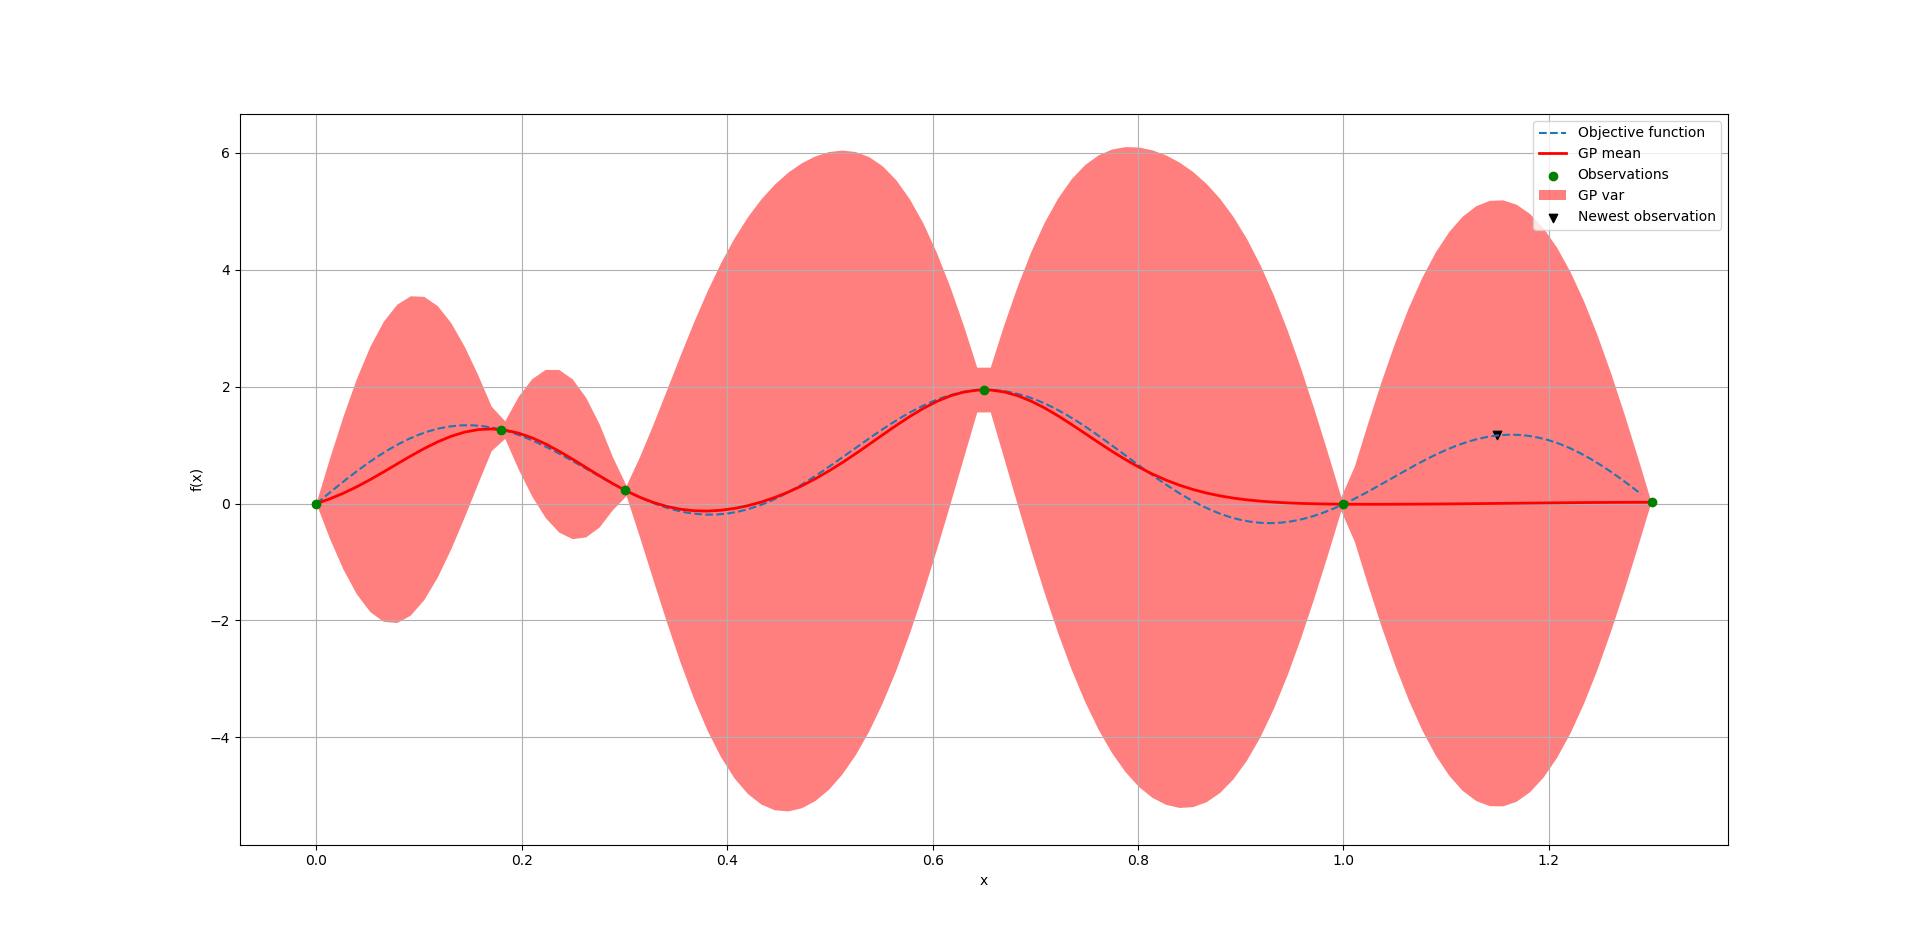
\includegraphics[width=\linewidth]{images/intro_images/BOLoop_4.png}}
    \only<5>{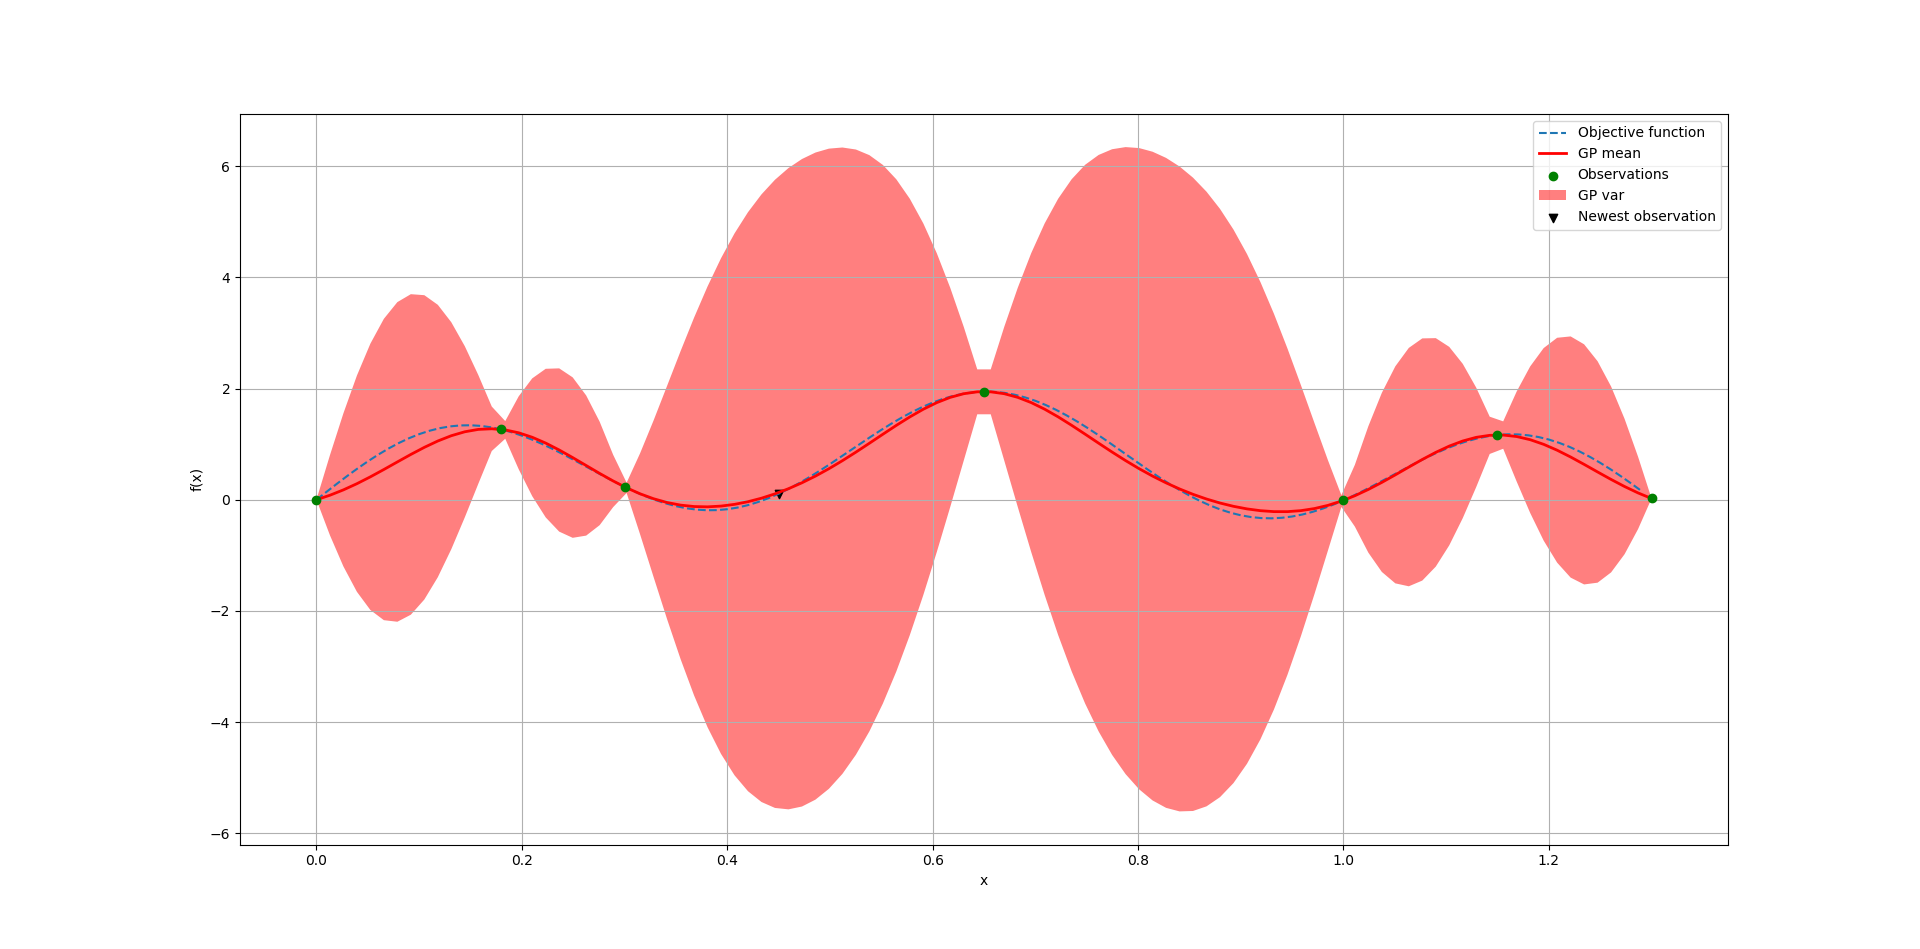
\includegraphics[width=\linewidth]{images/intro_images/BOLoop_5.png}}
    \only<6>{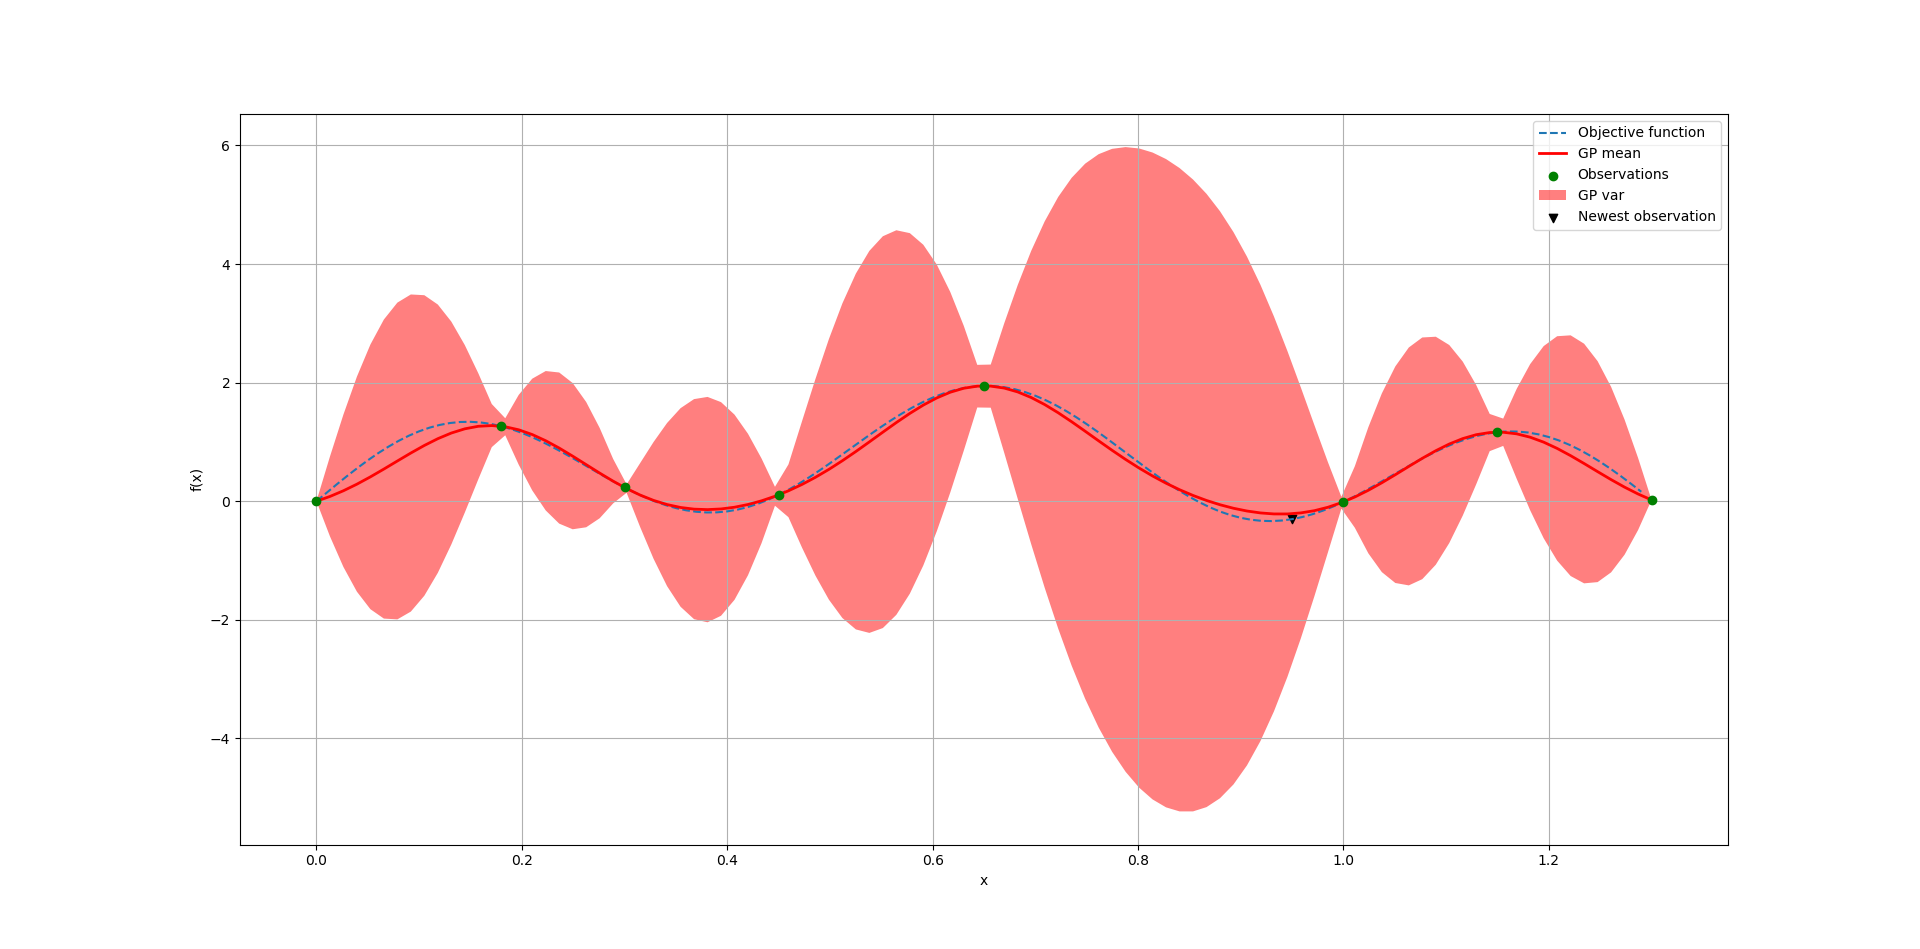
\includegraphics[width=\linewidth]{images/intro_images/BOLoop_6.png}}
    \only<7>{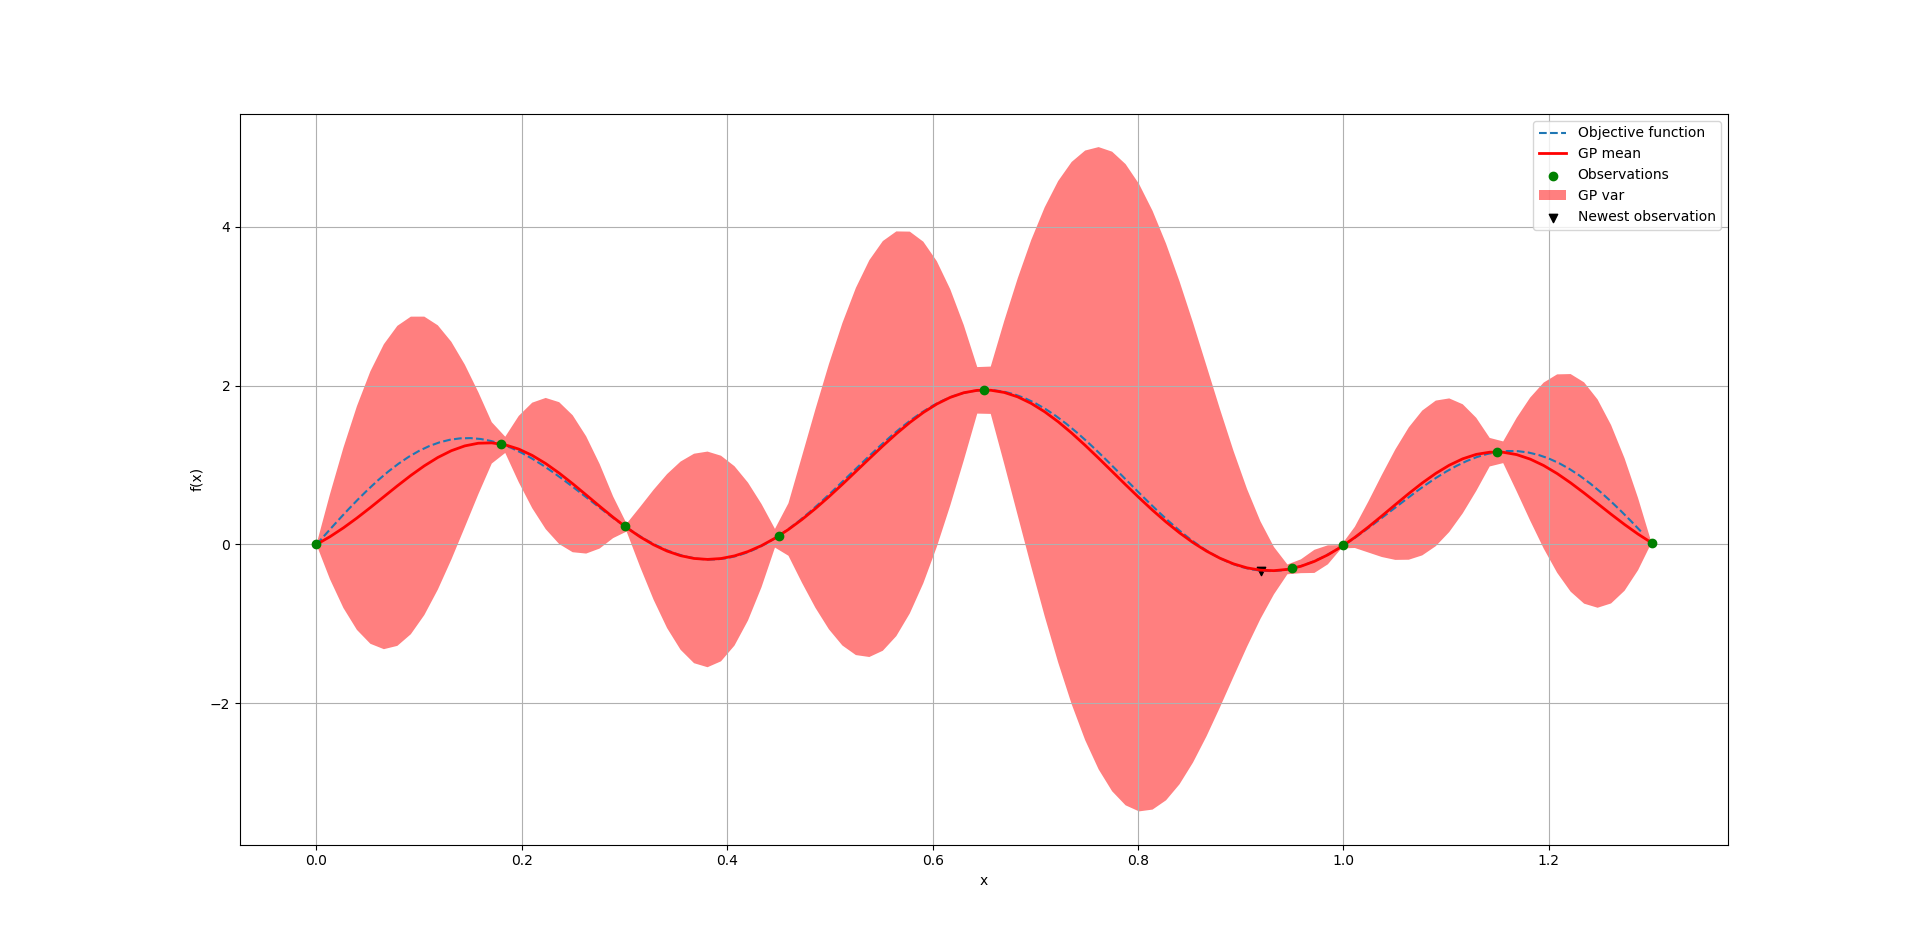
\includegraphics[width=\linewidth]{images/intro_images/BOLoop_7.png}}
    \only<8>{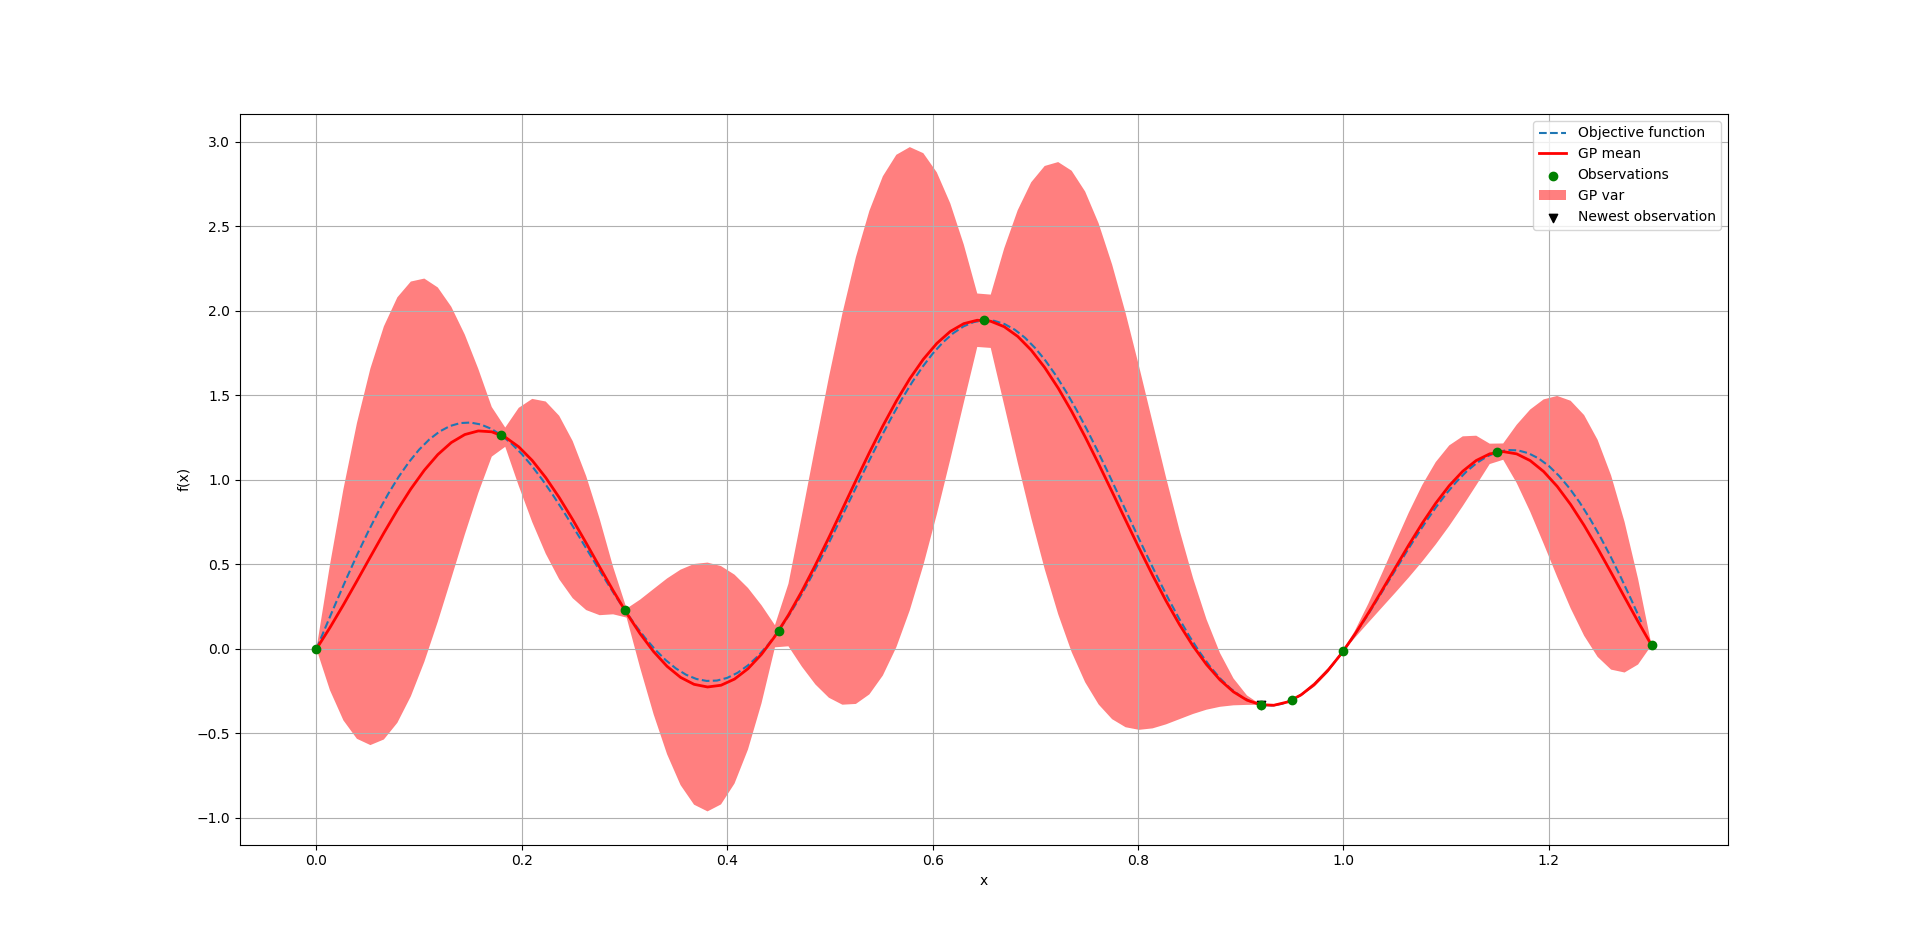
\includegraphics[width=\linewidth]{images/intro_images/BOLoop_8.png}}

\end{figure}


\end{frame}


%----------------------------------------------------------------------
\begin{frame}[c]{Bayesian Optimization: Pseudocode}
\begin{center}
\begin{minipage}{0.75\textwidth}
\begin{algorithm}[H]
    \Input{Search Space $\pcs$, 
    		black box function $\func$, 
    		acquisition function $\acq$, \\
    		maximal number of function evaluations $\bobudget$.
    	}
	\BlankLine
	$\dataset_0$ $\leftarrow$ initial\_design($\pcs$); 
	
	\For{\bocount = $1, 2, \ldots \bobudget - |\dataset_0|$}{
		%\While{$B$ not exhausted} {
		$\surro$ $\leftarrow$ fit predictive model on $\dataset_{\bocount-1}$;
		
		select $\bonextsample$ by optimizing $\bonextsample \in \argmax_{\conf \in \pcs} \acq(\conf; \dataset_{\bocount-1}, \surro)$;
		
		Query $\bonextobs := \func(\bonextsample)$;
		
		Add observation to data $\dataset_{\bocount} := \dataset_{\bocount-1} \cup \{\langle \bonextsample, \bonextobs \rangle \}$;\\
	}
	\Return{Best $\conf$ according to $\dataset_\bocount$ or $\surro$}
	\caption{BO loop}
\end{algorithm}
\end{minipage}
\end{center}
\note[item]{how to end lines?}
\end{frame}
%-----------------------------------------------------------------------



%----------------------------------------------------------------------
\begin{frame}[c]{Bayesian Optimization: Where does the name come from?}

\begin{itemize}
    \item Bayesian optimization uses Bayes' theorem: 
    	\begin{equation*}
    	    P(A \vert B) = \frac{P(B \wedge A) \times  P(A)}{P(B)}
    	    \propto P(B \vert A) \times  P(A)
    	\end{equation*} \pause
    \item We refer to:
        \begin{itemize}
            \item $A$ as a model (or hypothesis, theory), 
            \item $B$ as a data (or observations, evidence),
            \item $P(A \vert B)$ as a \emph{posterior} probability of a model given a data,
            \item $P(B \vert A)$ as a \emph{likelihood} of a data given a model, 
            \item $P(A)$ as a \emph{prior} probability of a model, which represents our belief about the space of possible objective functions. 
        \end{itemize}
    \item In our application:
        \begin{equation*}
            P(\func \vert \dataset_{1:\bocount}) \propto P(\dataset_{1:\bocount} \vert \func) * P(\func)
        \end{equation*} 
        where $\dataset_{1:\bocount} = \left \{ \conf_{1:\bocount}, \func(\conf_{1:\bocount}) \right \}$.

\end{itemize}

        
\end{frame}
%-----------------------------------------------------------------------

%----------------------------------------------------------------------

%-----------------------------------------------------------------------
\begin{frame}[c]{Bayesian Optimization: Advantages and Disadvantages}

\begin{columns}[T] % align columns
\begin{column}{.48\textwidth}

\only<1-9>{
    \begin{block}{Advantages}
    \begin{itemize}
      \item Sample efficient 
      \item Can handle noise
      \item Native incorporation of priors 
      \item Does not require gradients 
      \item Theoretical guarantees
      \item ...
    \end{itemize}
    \end{block}
}
\end{column}%

\hfill%

\begin{column}{.48\textwidth}
\only<4-9>{
    \begin{block}{Disadvantages}
    \begin{itemize}
      \item Overhead because of model training in each iteration 
      \item Open design choices: surrogate model, acquisition function 
      \myit{
      	\item Models need to take into account high dimensions, categorical dimensions, etc
      }
      \item Inherently sequential (in its basic form)
 %      \item Has hyperparameters of its own
    \end{itemize}
\end{block}
}
\end{column}
\end{columns}


\end{frame}
%-----------------------------------------------------------------------







%-----------------------------------------------------------------------
%----------------------------------------------------------------------
%\begin{frame}[c]{Surrogate modelling}
%\framesubtitle{General idea}
%\begin{itemize}
%    \item Use a surrogate model of the expensive function $\cost$ as a cheap-to-evaluate proxy.
%    \begin{itemize}
%        \item Use a probabilistic model with well-calibrated uncertainty predictions.
%    \end{itemize}
%    \pause
%    \item Define a utility function to guide the search for new data points.
%    \pause
%    \item Use the optimization of the utility function as a decision procedure to provide inference on where to evaluate next.
%
%\end{itemize}
%\end{frame}

%-----------------------------------------------------------------------